\chapter{Experimental results}\label{ch:experiments}

We have four different optimization algorithms to choose from:
\begin{itemize}
    \item \textit{EVO-STOPS} - an evolutionary algorithm that encodes a solution as a list of routes of stops and tries to improve the solution by modifying these routes.
    \item \textit{EVO-CR} - an evolutionary algorithm that encodes a solution using a mapping from groups from buses and an array defining the order of pick-ups and drop-offs.
    \item \textit{EVO-H} - an evolutionary algorithm that uses only mapping from groups to buses and creates the routes using a greedy heuristic.
    \item \textit{ACO} - iteratively creates new solutions using the \textit{Ant Colony Optimization} metaheuristic.
\end{itemize}

To compare the approaches, we generated benchmark datasets and ran all the algorithms on them. In this chapter, we present the results.

\section{Parameters}

All used datasets contain 100 passenger requests. Each group has between 1 and 10 people. The depot is always set in Prague. It is important to note that the first group in each route gets always picked up on time. This means that the location of the depot has no effect on the group's delays; setting it far from the departure area does, however, make using more buses more costly.

All the algorithms use the same fitness function, with the delay penalty constant equaling $0.01$. All genetic algorithms have $10\%$ of the population's best individuals (\textit{elites}) passed from the old to the new population. Other parameters are set as described in Sections \ref{sec:genetic_hyperparams} and \ref{sec:aco_hyperparams}.

All experiments were performed on an AMD EPYC 7532 processor with 6 GB of RAM available.

For all experiments, we include a plot showing the progression of the best fitness value found by each approach. The value shown is the mean best fitness of 10 different runs, with the first and third quartiles depicted by the translucent region. The figure shows progression in time and has both the x and y axis on a logarithmic scale. The statistics about the best solutions returned by each algorithm are described in two tables. First shows the basic information - total costs (in thousands), kilometers traveled in total, size of the delay penalties in the fitness function (in thousands) and how much of the fitness value they take, and the number of buses used. The second table shows information about group delays - the maximum delay of a group and the average and median delays of all groups, respectively.

\section{Commute dataset}

In the commute dataset, each customer group departs from a random location in Pilsen and travels to a random location in Prague. The distance between the two cities is approximately 90 kilometers. The departure times are randomly distributed in a four-hour time window. The available bus type can carry up to $80$ people, its operating cost per kilometer is $80$, and its fixed rental cost is $50000$. The algorithms ran for exactly 90 minutes, after which they were terminated.

The upper limit of buses used for genetic algorithms was set to $30$. The \textit{ACO} algorithm has no such limit.

When examining the results, we see that the \textit{ACO} performed the worst, since it failed to minimize the number of buses used. This resulted in the highest total costs and the greatest number of kilometers traveled. All genetic algorithms returned similar results. \textit{EVO-CR} minimized the total costs the most while \textit{EVO-H} handled the group delays slightly better.

\clearpage

\begin{figure}
    \centering
    \includegraphics[width=1\linewidth]
    {img/exp_commute_100_time.pdf}
    \caption{Commute dataset - Fitness values in time}
    \label{fig:exp_commute}
\end{figure}

\begin{table}
    \centering
    \begin{tabular}{lcccccc}
         & Total costs & Distance traveled & Delay penalties & Buses used \\
         \hline
         EVO-STOPS & 2149 & 8732 km & 612 (22\%) & \textbf{29} \\
         EVO-CR & \textbf{2140} & \textbf{8626 km} & 524 (20\%) & \textbf{29} \\
         EVO-H & 2240 & 9255 km & \textbf{429 (16\%)} & 30 \\
         ACO-HCF & 2822 & 12147 km & 472 (14\%) & 37 \\
    \end{tabular}
    \caption{Commute dataset - Route statistics}
    \label{tab:exp_commute_route_stats}
\end{table}

\begin{table}
    \centering
    \begin{tabular}{lcccccc}
         &  Maximum delay & Average delay & Median delay \\
         \hline
         EVO-STOPS & 30m25s & 11m26s & 11m21s \\
         EVO-CR & 28m2s & 10m10s & 10m26s \\
         EVO-H & \textbf{23m3s} & 9m5s & 8m56s \\
         ACO-HCF & 37m2s & \textbf{7m36s} & \textbf{5m1s} \\
    \end{tabular}
    \caption{Commute dataset - Delay statistics}
    \label{tab:exp_commute_delay_stats}
\end{table}

\clearpage

\section{Uniformly distributed dataset}

The uniformly distributed data set has both departure and destination points scattered randomly throughout Prague, and departure times are also randomly distributed within a 5-hour time window. The available bus type can carry up to $40$ people, its operating cost per kilometer is $60$, and its fixed rental cost is $30000$. The wall time was set to 90 minutes.

\subsection{25 buses}

When the upper limit of buses for genetic algorithms is set to $25$, the \textit{ACO} clearly outperforms all other approaches, as the limit is set too high. \textit{EVO-CR} struggled the most with lowering the buses used, resulting in the highest overall costs. We can also see that \textit{EVO-STOPS} fails the most in dealing with delay penalties, which are higher than for the \textit{ACO} while using $5$ more buses. \textit{EVO-H} found a solution with minimal group delays, with the maximum delay being under 4 minutes.

\subsection{16 buses}

Lowering the upper limit for buses to 16 greatly improves the performance of all genetic algorithms. However, the \textit{ACO} still managed to minimize the total costs the most. \textit{EVO-STOPS} performed the worst in all aspects. \textit{EVO-CR} and \textit{EVO-H} performed similarly, with \textit{EVO-CR} using a bus more, but having slightly shorter delays. The \textit{ACO} run is the same as in the previous experiment.

\clearpage

\begin{figure}
    \centering
    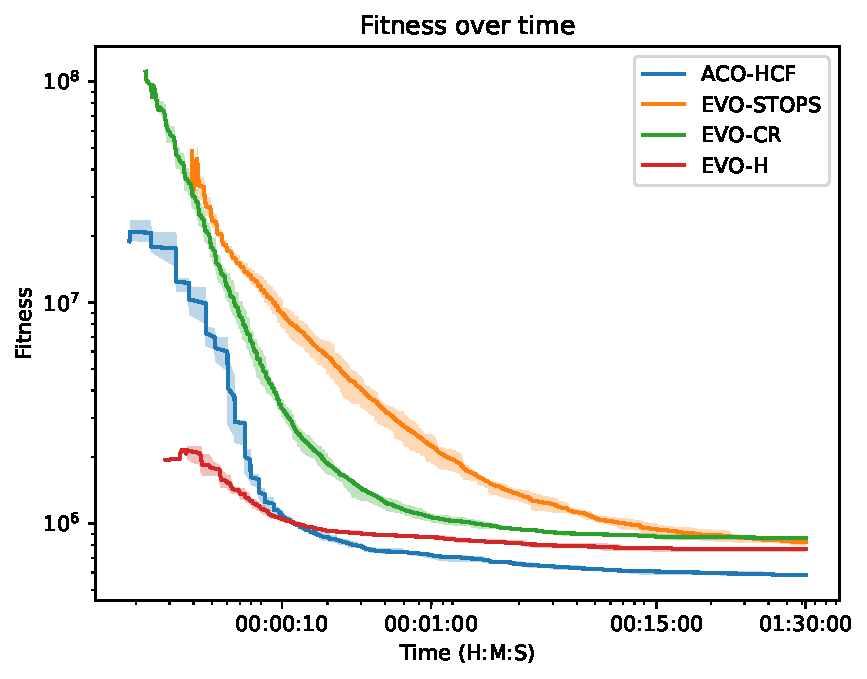
\includegraphics[width=1\linewidth]
    {img/exp_random_25b_100_time.pdf}
    \caption{Uniformly distributed dataset, 25 buses limit - Fitness values in time}
    \label{fig:exp_random_25}
\end{figure}

\begin{table}
    \centering
    \begin{tabular}{lcccccc}
         & Total costs & Distance traveled & Delay penalties & Buses used \\
         \hline
         EVO-STOPS & 732 & 2698 km & 18.9 (2\%) & 19 \\
         EVO-CR & 807 & 2458 km & 1.3 (0\%) & 22 \\
         EVO-H & 718 & 2459 km & \textbf{0.9 (0\%)} & 19 \\
         ACO-HCF & \textbf{566} & \textbf{2431 km} & 14.6 (3\%) & \textbf{14} \\
    \end{tabular}
    \caption{Uniformly distributed dataset, 25 buses limit - Route statistics}
    \label{tab:exp_random_25_route_stats}
\end{table}

\begin{table}
    \centering
    \begin{tabular}{lcccccc}
         &  Maximum delay & Average delay & Median delay \\
         \hline
         EVO-STOPS & 13m26s & 35s & \textbf{0s} \\
         EVO-CR & 4m18s & 7s & \textbf{0s} \\
         EVO-H & \textbf{3m52s} & \textbf{5s} & \textbf{0s} \\
         ACO-HCF & 11m54s & 41s & \textbf{0s} \\
    \end{tabular}
    \caption{Uniformly distributed dataset, 25 buses limit - Delay statistics}
    \label{tab:exp_random_25_delay_stats}
\end{table}

\clearpage

\clearpage

\begin{figure}
    \centering
    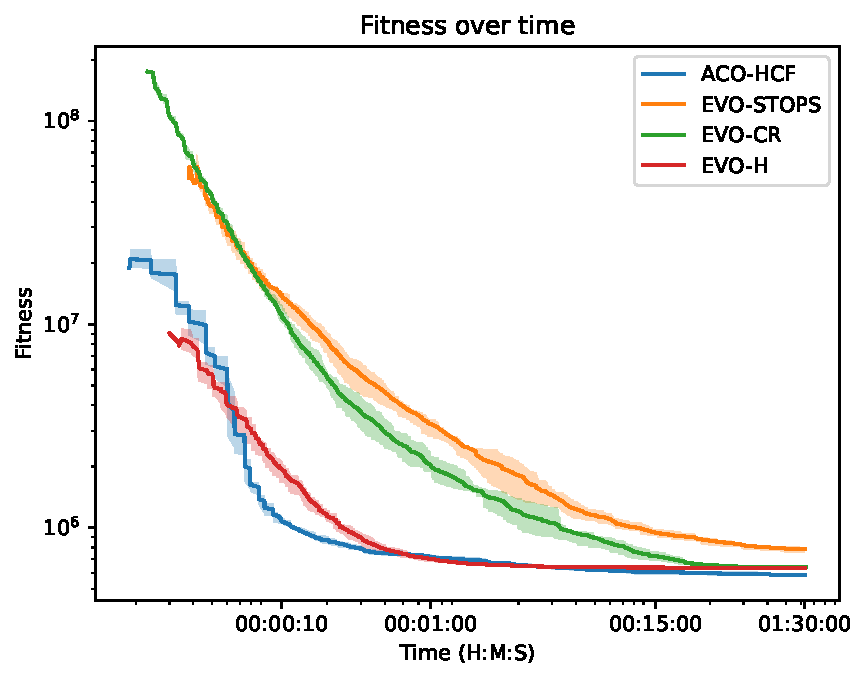
\includegraphics[width=1\linewidth]
    {img/exp_random_16b_100_time.pdf}
    \caption{Uniformly distributed dataset, 16 buses limit - Fitness values in time}
    \label{fig:exp_random_16}
\end{figure}

\begin{table}
    \centering
    \begin{tabular}{lcccccc}
         & Total costs & Distance traveled & Delay penalties & Buses used \\
         \hline
         EVO-STOPS & 635 & 2577 km & 108 (15\%) & 16 \\
         EVO-CR & 626 & 2440 km & \textbf{6 (1\%)} & 16 \\
         EVO-H & 597 & 2443 km & 9 (1\%) & 15 \\
         ACO-HCF & \textbf{566} & \textbf{2431 km} & 15 (3\%) & \textbf{14} \\
    \end{tabular}
    \caption{Uniformly distributed dataset, 16 buses limit - Route statistics}
    \label{tab:exp_random_16_route_stats}
\end{table}

\begin{table}
    \centering
    \begin{tabular}{lcccccc}
         &  Maximum delay & Average delay & Median delay \\
         \hline
         EVO-STOPS & 28m15s & 2m12s & \textbf{0s} \\
         EVO-CR & \textbf{8m19s} & \textbf{23s} & \textbf{0s} \\
         EVO-H & 8m33s & 30s & \textbf{0s} \\
         ACO-HCF & 11m54s & 41s & \textbf{0s} \\
    \end{tabular}
    \caption{Uniformly distributed dataset, 16 buses limit - Delay statistics}
    \label{tab:exp_random_16_delay_stats}
\end{table}

\clearpage

\section{Combined dataset}

Finally, we combined both types of requests in a \textit{combined dataset}. Approximately half of the
$100$ customers travel between Prague and Pilsen, while the other half travels either within Pilsen or Prague. Departure times are distributed randomly within a 4-hour time window. The available bus type has a capacity of $80$ persons, its operating cost per kilometer is $80$, and its fixed cost for rental is $50000$. The upper limit for buses used for genetic algorithms was set to $20$. The wall time was set to $120$ minutes.

The performance of each algorithm reflects its performance in both previous datasets. The \textit{ACO} performed the worst. When inspecting the best solution returned, it can be seen that the algorithm had the most trouble with the commute requests, most of the time failing to pick up multiple customers before traveling between the cities. This resulted in the highest number of buses used. However, it performed well with the requests within each of the cities, with the median delay being zero seconds. The genetic algorithms then performed surprisingly similarly. \textit{EVO-CR}
managed to lower the total costs the most, while \textit{EVO-H} dealt the best with group delays. Both of the algorithms have the same maximum delay, which belongs to the same group.

\clearpage

\begin{figure}
    \centering
    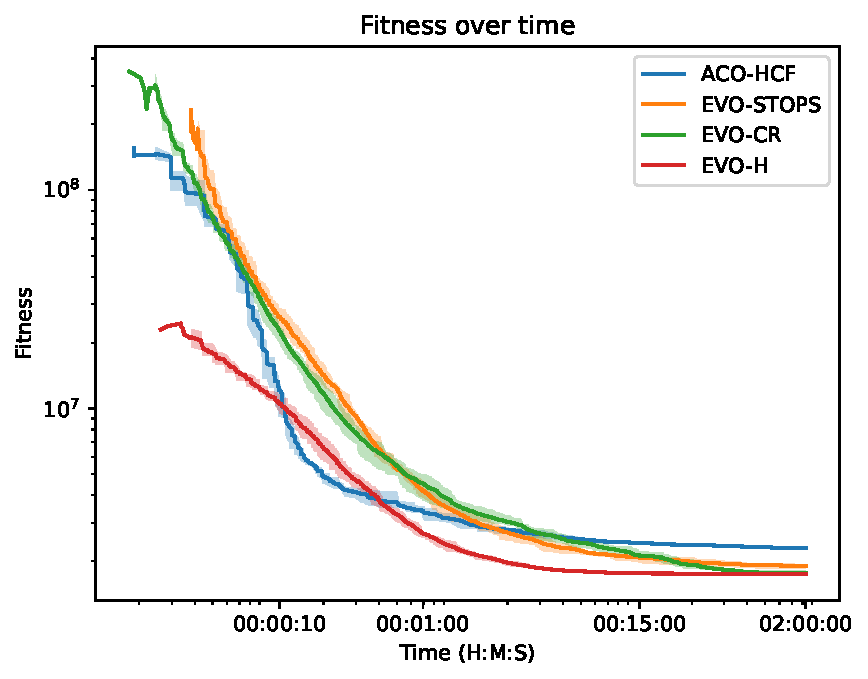
\includegraphics[width=1\linewidth]
    {img/exp_mixed_100_time.pdf}
    \caption{Mixed dataset - Fitness values in time}
    \label{fig:exp_mixed}
\end{figure}

\begin{table}
    \centering
    \begin{tabular}{lcccccc}
         & Total costs & Distance traveled & Delay penalties & Buses used \\
         \hline
         EVO-STOPS & 1597 & 6833 km & 219 (12\%) & 21 \\
         EVO-CR & \textbf{1522} & \textbf{6528 km} & 194 (11\%) & 20 \\
         EVO-H & 1529 & 6613 km & \textbf{159 (9\%)} & \textbf{20} \\
         ACO-HCF & 2060 & 9501 km & 174 (8\%) & 26 \\
    \end{tabular}
    \caption{Mixed dataset - Route statistics}
    \label{tab:exp_mixed_route_stats}
\end{table}

\begin{table}
    \centering
    \begin{tabular}{lcccccc}
         &  Maximum delay & Average delay & Median delay \\
         \hline
         EVO-STOPS & \textbf{21m23s} & 5m15s & 3m18s \\
         EVO-CR & 21m47s & 4m43s & 2m6s \\
         EVO-H & 21m47s & \textbf{2m5s} & 15s \\
         ACO-HCF & 34m11s & 2m50s & \textbf{0s} \\
    \end{tabular}
    \caption{Mixed dataset - Delay statistics}
    \label{tab:exp_mixed_delay_stats}
\end{table}

\clearpage